%!TEX root = ../../../main.tex
\section{Navigation} % (fold)
\label{sec:mr_navigation}


    \subsection{Relative navigation} % (fold)
    \label{sub:mr_relative_navigation}
    Making use of the combined odometry from the wheels and the IMU, the relative navigation has been implemented
    % subsection relative_navigation (end)



    \subsection{Line navigation} % (fold)
    \label{sub:mr_line_navigation}
    
    % subsection line_navigation (end)



    \subsection{Free navigation} % (fold)
    \label{sub:mr_free_navigation}
    
    As per project description, the navigation inside the box is to be done based on SLAM. 
    Due to complexity of the entire project and potential diversity of SLAM implementations, an open-source implementation of SLAM was chosen. 
    More specifically the gmapping-package \cite{gmapping} which has a livid community of supporters and builds a ROS wrapper for “OpenSlam's Gmapping”\cite{openslam}. 
    TF-Frames of Lidar, IMU and the robot base were set up, this allows for easy transformation between Lidar and odometry data, inside the package. 
    Using these, the SLAM-Implementation uses a particle filter to sequentially build up a map of the area. 
    By manually driving through the entire workspace, a map was created. 
    \begin{figure}[H]
        \centering
        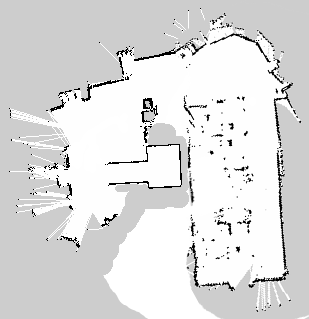
\includegraphics[width=0.5\textwidth]{slam_map}
        \caption{Slam Map}
        \label{fig:slam_map}
    \end{figure}
    Using the map-server package from the ROS 2D-Navigation Stack \cite{navigation_stack} the generated map was stored and is then broadcasted as a static map for localization. 
    The AMCL (Adaptive Monte-Carlo Localization) package (which is also included in the navigation stack) then uses the static map, the LIDAR as well as odometry data to localize the robot while in free navigation. 
    After tuning the parameters, AMCL worked fairly reliably for navigation both inside and outside the box.\\
    \textbf{TODO: Describe move{\_}base}\\
    Due to the box being fairly monotone in respect to the LIDAR readings (clean, walls, no landmarks), precise navigation inside the box was sometimes not perfect. 
    Also with multiple robots present in the box, issues, especially when trying to charge occurred. 
    To ensure reliability of charging, a backup behavior was added, when the charging failed using move{\_}base. 
    For this a line was added, using the already implemented Line Following behavior. 
    The move{\_}base is used to navigate the robot to the start of the charging line. 
    Then the robot follows the line until a pre-specified distance from the wall using LIDAR. 
    Having a main and a backup behavior proved to be sufficient for reliable charging\\
    \textbf{TODO: IS THAT REALLY SO?}

    % subsection free_navigation (end)

% section navigation (end)